\chapter{Applicazione di SFA: La Tramvia di Firenze}
In questo capitolo verr\`a analizzata una particolare applicazione di SFA al problema del posizionamento ferrotramviario.\\*
Nell'ambito di un progetto di ricerca finanziato dall'Unione Europea, si \`e voluto studiare l'usabilit\`a di SFA come sistema di posizionamento ferrotramviario alternativo a quello descritto nel Capitolo 1, il quale fa un largo uso di apparati installati a terra, fatto che si vorrebbe minimizzare.\\*
L'idea di base \`e quella di utilizzare UKF per stimare la posizione del treno attraverso misure di accelerazione, velocit\`a angolare, velocit\`a lineare e posizione. La rilevazione di tali grandezze, per quanto esposto nel Capitolo 2, \`e caratterizzata da rumore, UKF combina queste informazioni per stimare la posizione del treno al netto dei rumori di processo e dei rumori di misura.
\section{Architettura di Sistema}
Il sistema progettato ha lo scopo di eseguire SFA su una piattaforma hardware installata bordo treno, la quale riceve i dati \emph{raw} dai sensori e li elabora al fine di stimare la progressiva chilometrica del treno in ciascun istante di tempo.\\*
Tale posizione sar\`a inviata, attraverso un modem \texttt{LTE}:
\begin{itemize}
	\item All'OBCU, per essere utilizzata attivamente all'interno del sistema di \emph{interlocking}
	\item Ad un arbitario host che esegue un software grafico di tracciamento del treno: il \texttt{RailTrackTool} (RTT)
\end{itemize}
\`E possibile descrivere l'architettura di sistema a due differenti livelli: architettura a livello \emph{hardware} e architettura a livello \emph{software}.
\subsection{Architettura Hardware}
Sul treno \`e stata installata una scheda \texttt{Nvidia TX-Jetson} quale piattaforma di elaborazione dei dati. I sensori atti a campionare le misurazioni sono stati collegati alla scheda mediante appositi bus dati.\\*
Il \emph{sensor set} utilizzato in quest'applicazione \`e composto dai seguenti sensori:
\begin{itemize}
	\item \emph{Inertial Measurement Unit} (IMU):\\*
	Sensore incaricato di misurare i vettori \texttt{accelerazione} ($\mathbf{a}$) e \texttt{velocit\`a angolare} ($\mathbf{v_{ang}}$) attraverso l'uso combinato di un accelerometro e un giroscopio. Le misure di IMU sono prese rispetto alla Terra\footnote{Approssimata come un \emph{sistema inerziale}.} e sono espresse in unit\`a stabilite dallo standard internazionale (SI):
	$$
	\mathbf{a}\;\left[\frac{m}{s^2}\right]\;\;\;\;\mathbf{v_{ang}}\;\left[ \frac{rad}{s} \right]
	$$Si tratta del sensore principale su cui si basa l'esecuzione di SFA.\\*
	IMU \`e caratterizzato da un rumore di misura tale per cui, se venisse utilizzato esclusivamente come sorgente di aggiornamento del filtro,
	la stima della posizione risulta caratterizzata da un \emph{drift lineare}, il quale fa discostare il valore di posizione stimata da quello reale, in una quantit\`a che \`e funzione lineare del tempo.\\*
	\begin{figure}[h]
		\centering
		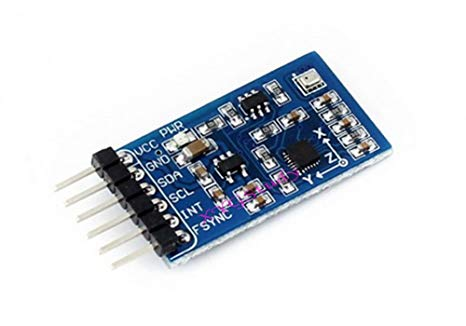
\includegraphics[width=\linewidth]{img/imu}
		\caption{\emph{Inertial Measurment Unit}}
		\label{fig:imu}
	\end{figure}
	\item Odometro:\\*
	Per realizzare l'odometro \`e stato installato un rilevatore radar su una ruota del treno. Il radar misura il tempo impiegato dalla ruota a compiere un giro completo, e determina la velocit\`a angolare della ruota $\varphi'(t) = \frac{2\pi}{tempo} \left[ \frac{rad}{s}\right]$.\\*
	Noto il raggio $r\;[m]$ della ruota, \`e possibile determinare la velocit\`a lineare alla circonferenza della ruota  $x'(t)$ attraverso la relazione cinematica $x'(t) = -r\varphi'(t) \left[ \frac{m\;rad}{s}\right] = -r\varphi'(t) \left[ \frac{m}{s} \right]$.\\*
	Approssimando il treno come un \emph{corpo rigido}, questa sar\`a la velocit\`a lineare con cui il treno si sta muovendo.
	\item Global Positioning System (GPS):\\*
	Sensore che riceve i dati di posizione attraverso il sistema satellitare GPS.\\*
	Le misure di GPS sono riportate in formato standard come tripla di coordinate \texttt{(latitudine, longitudine, altitudine)}, rispettivamente espresse in gradi \texttt{N-S}, in gradi \texttt{E-O} e in \texttt{metri}.\\*
	In generale queste misure sono le meno affidabili in quanto la \emph{varianza} della variabile aleatoria che modella tale sorgente \`e la pi\`u significativa.
\end{itemize}
 Ad una data frequenza, i sensori inviano dati verso la scheda; quest'ultima, dopo aver eseguito un'iterazione di SFA\footnote{Ossia, un \emph{aggiornamento} di UKF}, invia a OBCU (e/o a RTT) la stima della posizione del treno attraverso apposita modulazione di segnale elettromagnetico, in accordo con il protcollo \texttt{LTE}. Lo schema riportato in figura \ref{fig:tdiagram} mostra un diagramma dell'architettura hardware appena descritta.
\begin{figure}[h]
	\centering
	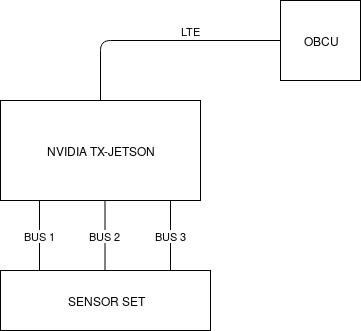
\includegraphics[width=0.7\linewidth]{img/TrainDiagram}
	\caption{Architettura hardware bordo treno}
	\label{fig:tdiagram}
\end{figure}
\subsection{Architettura Software}
Sulla scheda \`e installato il sistema operativo \texttt{Ubuntu 16.04 LTS}, basato su kernel \texttt{Linux}.\\*Qualunque software menzionato in questa Tesi \`e stato sviluppato in linguaggio \texttt{C++}.\\*
Un set di tre moduli software, denominati \texttt{interface-modules}, sono in esecuzione sulla scheda.\\*
Sia MOD\_$i$ l'$i-$esimo modulo software del set e SERIAL\_$i$ l'$i-$esima interfaccia seriale della scheda, per $i = 1,2,3$.\\*
Il funzionamento di \texttt{interface-modules} \`e il seguente:
\begin{itemize}
	\item IMU invia la coppia \texttt{(accelerazione,velocit\`a angolare)} a SERIAL\_1, MOD\_1 legge i valori da SERIAL\_1 e li invia a un secondo modulo software, denominato \texttt{listener}, attraverso l'interfaccia di rete \texttt{loopback}, in quanto \texttt{listener} esegue anch'esso sulla scheda;
	\item Odometro invia il valore di \texttt{velocit\`a lineare} a SERIAL\_2, MOD\_2 legge i valori da SERIAL\_2 e li invia a \texttt{listener};
	\item GPS invia i valori di \texttt{(latitudine, longitudine, altitudine)} a SERIAL\_3, MOD\_3 legge i valori da SERIAL\_3 e li invia a \texttt{listener}.
\end{itemize}
La comunicazione fra \texttt{interface-modules} e \texttt{listener} avviene attraverso un protocollo applicazione stabilito arbitrariamente, sia esso \texttt{INPUT\_PROTOCOL}, mentre a livello di trasporto si utilizza \texttt{UDP}.\\*
I valori ricevuti da \texttt{listener} vengono salvati in apposite \emph{strutture dati} rappresentanti misure della stessa sorgente:
\begin{itemize}
\item I vettori accelerazione e velocit\`a angolare rilevati da IMU vengono convertiti nella struttura dati \texttt{IMU\_POD};
\item La velocit\`a rilevata dal Radar/Odometro viene convertita nella struttura dati \texttt{ODO\_POD};
\item La posizione rilevata dal GPS viene infine convertita nella struttura dati \texttt{GPS\_POD}.
\end{itemize}
Il software che esegue effettivamente SFA \`e compilato come una libreria, \texttt{FusionLib}, utilizzata da \texttt{listener}. \texttt{FusionLib} dispone di interfacce software in entrata e in uscita, ossia \texttt{listener} \`e in grado di inviare le misurazioni a SFA, quali variabili di tipo \texttt{IMU\_POD, ODO\_POD, GPS\_POD} ed altres\'i di ricevere la stima della posizione del treno, essendo questo l'output dell'algoritmo, quale variabile di tipo \texttt{SFA\_OUTPUT\_POD}.\\*
Ogniqualvolta \texttt{listener} riceva un' uscita da SFA, si fa carico della comunicazione tra scheda e OBCU/RTT. Questa comunicazione, fisicamente possibile attraverso l'utilizzo del modem \texttt{LTE}, avviene utilizzando un protocollo di rete arbitrario a livello applicazione, sia esso \texttt{OUTPUT\_PROTOCOL}, mentre al livello di trasporto la scelta \`e nuovamente ricaduta su \texttt{UDP} per ragioni di efficienza.\\*
Uno schema dell'architettura software \`e quello mostrato in figura \ref{fig:tdiagramint}.\\*
\begin{figure}[h]
	\centering
	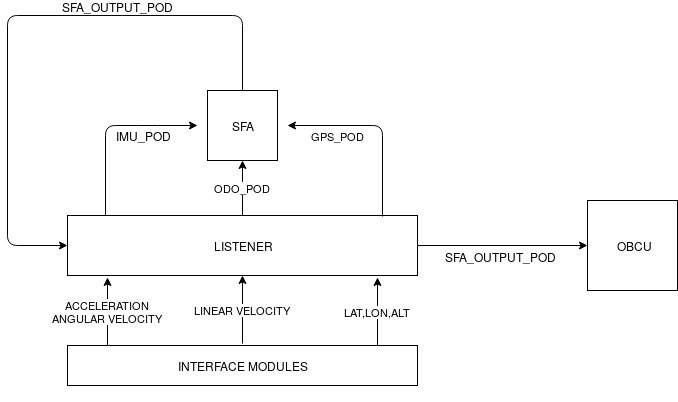
\includegraphics[width=\linewidth]{img/InternalTrainSchema}
	\caption{Architettura software bordo treno}
	\label{fig:tdiagramint}
\end{figure}
\section{Gestione della trasmissione dei dati}
Nella precedente sezione sono stati brevemente introdotti i protocolli di comunicazione implementati per gestire la comunicazione \texttt{UDP}:
\begin{itemize}
	\item In entrata, tra \texttt{interface-modules} e \texttt{listener} (\texttt{INPUT\_PROTOCOL});
	\item In uscita, tra \texttt{listener} e OBCU/RTT (\texttt{OUTPUT\_PROTOCOL}).
\end{itemize}
\subsection{Trasmissione in entrata}
Per trasmettere i dati da \texttt{interface-modules} a \texttt{listener}, e dunque dai sensori al modulo software che implementa SFA, \`e stato realizzato un protocollo di comunicazione denominato \texttt{INPUT\_PROTOCOL}.\\*
Tale protocollo fa affidamento a livello trasporto su \texttt{UDP} per massimizzare la velocit\`a di trasmissione senza dover necessariamente rinunciare all'integrit\`a dei messaggi trasmessi, in quanto la comunicazione avviene tra processi in esecuzione sulla stessa macchina, e la probabilit\`a che un messaggio venga perso o che questo venga ricevuto con errori, \`e assolutamente trascurabile.\\*
Il protocollo definisce il formato del \emph{payload} del pacchetto \texttt{UDP} che contiene le informazioni di IMU, Radar/Odometro, o GPS, ed \`e descritto in tabella \ref{tab:protoin}.\\*
\begin{table}[h]
			\centering
\begin{tabular}{|c|c|c|c|}
	\hline 
	\textbf{Campo} & \textbf{Descrizione} & \textbf{Indici di bit} & \textbf{Tipo} \\ 
	\hline 
	\texttt{SENSOR\_TYPE} & ID Sensore Sorgente & 0-7 & \texttt{uint8\_t} \\ 
	\hline 
	\texttt{Seq.NO} & Numero di sequenza & 8-23 & \texttt{uint16\_t} \\ 
	\hline 
	\texttt{N\_INT} & Numero di interi trasmessi & 24-31 & \texttt{uint8\_t} \\ 
	\hline 
	\texttt{N\_DOUBLE} & Numero di double trasmessi & 31-38 & \texttt{uint8\_t} \\ 
	\hline 
\end{tabular} 
\caption{Protocollo di comunicazione in entrata}
\label{tab:protoin}
\end{table}
A discrezione del valore del campo \texttt{SENSOR\_TYPE} si distingue il tipo di informazione trasportata dal pacchetto, come descritto in tabella \ref{tab:sensors}.\\*
\begin{table}[h]
		\centering
	\begin{tabular}{|c|c|}
		\hline 
		\textbf{Valore di SENSOR\_TYPE} & \textbf{Sorgente del pacchetto} \\ 
		\hline 
		$1$ & IMU \\ 
		\hline 
		$2$ & ODOMETRO \\ 
		\hline 
		$3$ & GPS \\ 
		\hline 
		$8$ & GROUND TRUTH \\ 
		\hline 
		$9$ & STROBE \\ 
		\hline 
		$10$ & STOP \\ 
		\hline 
	\end{tabular} 
	\caption{Significato del campo SENSOR\_TYPE}
	\label{tab:sensors}
\end{table}
I pacchetti \texttt{GROUND TRUTH} sono pacchetti di inizializzazione dell'algoritmo: alla ricezione del pacchetto \texttt{GROUND TRUTH} l'algoritmo si avvia leggendo i valori trasmessi in coda al pacchetto, in accordo al valore dei campi \texttt{N\_INT} e \texttt{N\_DOUBLE}. Tali valori forniscono informazioni come progressiva chilometrica e velocit\`a iniziali del treno.\\*
I pacchetti \texttt{STROBE} sono inviati ogni secondo e forniscono un solo valore \texttt{double}, ossia un \texttt{timestamp} che l'algoritmo utilizza per sincronizzarsi.\\*
Il pacchetto \texttt{STOP} non contiene alcuna informazione utile: indica soltanto all'algoritmo di terminare l'esecuzione.\\*
Alla ricezione di un pacchetto, \texttt{listener} legge il valore del campo\\*\texttt{SENSOR\_TYPE}, e costruisce, in accordo alla relazione sorgente-struttura dati, la variabile da inviare a SFA.\\*
Il corretto ordinamento dei pacchetti trasmessi a SFA \`e garantito attraverso l'esplicito utilizzo di un buffer, codificato all'interno di \texttt{listener}, in cui i pacchetti vengono temporaneamente salvati prima di essere inviati a SFA, ed eventualmente ordinati sulla base del valore del campo \texttt{Seq.NO}.\\*
Si osservi che se l'integrit\`a non \`e minacciata dall'utilizzo di \texttt{UDP} quale protocollo di trasporto fra processi all'interno della stessa macchina fisica, altrettanto non si pu\`o dire dell'ordinamento dei messaggi. Questi potrebbero subire dei ritardi casuali in base allo stato del sistema operativo, in particolare lo \emph{scheduling} dei processi pu\`o avere influenze determinanti sullo scorretto ordinamento dei messaggi trasmessi. Utilizzando \texttt{TCP} si ovvierebbe a questa problematica, ma l'overhead insito nel protocollo stesso causerebbe un notevole degrado delle performance di SFA.
\subsection{Trasmissione in uscita}
La trasmissione dei dati in uscita da SFA avviene, in accordo al protocollo \texttt{OUTPUT\_PROTOCOL} tra \texttt{listener} e OBCU, o comunque, tra \texttt{listener} e qualunque host arbitrario che intenda ricevere le informazioni in uscita, come ad esempio un \texttt{PC} sul quale viene eseguito RTT.\\*
Come specificato, la comunicazione \`e posta in essere, a livello fisico, attraverso il protocollo \texttt{LTE}, ossia un un protocollo \emph{wireless}; mentre a livello trasporto si \`e scelto di continuare a usare \texttt{UDP} in luogo di \texttt{TCP}, col fine di massimizzare le \emph{performance} del sistema.\\*Il rischio di ricevere alcune informazioni in maniera errata, o non riceverle del tutto, \`e nettamente pi\`u elevato rispetto allo scenario precedente, nel caso in cui lo spazio fisico attraverso cui si propaga il segnale \texttt{LTE} \`e tale per cui quest'ultimo venga disturbato da sorgenti esterne.\\* Gli effetti deleteri di questa condizione sono particolarmente osservabili in alcuni tratti della linea ferrotramviaria, dove possono essere presenti numerose abitazioni e mezzi di trasporto in strada che si interpongono fisicamente tra la scheda \texttt{NVidia TX-Jetson} su cui esegue SFA e l'arbitrario host su cui viene eseguito RTT.\\*Occorre tuttavia osservare che il tracciamento del treno tramite RTT non \`e in alcun modo legato alla \emph{safety} del sistema, in quanto le funzionalit\`a \emph{safety-critical} riguardano la comunicazione tra la scheda e OBCU, ossia tra la scheda e il sistema di \emph{interlocking}.\\*
Questa problematica \`e risolta attraverso l'esplicito utilizzo di un meccanismo di \texttt{acknowledgment} simile a quello utilizzato da \texttt{TCP}: ciascun pacchetto in uscita da SFA viene indicizzato con un \emph{sequence number} e, in ricezione, viene inviato ogni secondo un \emph{ack} replicante l'ultimo numero di sequenza correttamente ricevuto. Solo quando il mittente riceve l'ack $i$ dal destinatario invier\`a il messaggio contenente l'uscita indicizzata con \emph{sequence number} $i+1$.\\*
Anche in questo caso, il protocollo definisce il formato del \emph{payload} del pacchetto \texttt{UDP} inviato da \texttt{listener}, ed \`e riportato in tabella \ref{tab:protoout}.\\*
\begin{table}[h]
	\centering
	\begin{tabular}{|c|c|c|c|}
		\hline 
		\textbf{Campo} & \textbf{Descrizione} & \textbf{Indici di bit} & \textbf{Tipo} \\ 
		\hline
		\texttt{Seq.NO} & Numero di sequenza & 0-15 & \texttt{uint16\_t} \\ 
		\hline 
		\texttt{ECEF\_X} & Coordinata X del treno & 16-79 & \texttt{double} \\ 
		\hline 
		\texttt{ECEF\_Y} & Coordinata Y del treno & 80-143 & \texttt{double} \\ 
		\hline 
		\texttt{ECEF\_Z} & Coordinata Z del treno & 144-207 & \texttt{double} \\ 
		\hline 
		\texttt{FU\_ARC\_LEN} & Progressiva chilometrica & 208-271 & \texttt{double} \\ 
		\hline 
	\end{tabular} 
\caption{Protocollo di comunicazione in uscita}
\label{tab:protoout}
\end{table}
In ricezione dovr\`a essere inviato il pacchetto \emph{ack} al mittente, ed il suo formato \`e descritto in tabella \ref{tab:ack}.
\begin{table}[h]
	\centering
	\begin{tabular}{|c|c|c|c|}
	\hline 
	\textbf{Campo} & \textbf{Descrizione} & \textbf{Indici di bit} & \textbf{Tipo} \\ 
	\hline
	\texttt{ACK} & Ultimo \texttt{Seq.NO} & 0-15 & \texttt{uint16\_t} \\ 
	\hline
\end{tabular}
\caption{Formato del pacchetto di \emph{ack}}
\label{tab:ack}
\end{table}
Si osserva che SFA produce la stima della posizione del treno sia in termini di progressiva chilometrica che di coordinate \texttt{ECEF}.\\*
\texttt{ECEF} \`e acronimo di \emph{Earth Centered Earth Fixed} ed \`e uno standard che misura le coordinate geografiche di un oggetto come la terna $ P = (x,y,z)$. Ciascuna coordinata viene espressa considerando la \emph{proiezione su piano} della Terra, e prendendo come origine $O$ l'intersezione fra l'equatore e il meridiano di \emph{Greenwich}.\\*
Le coordinate \texttt{ECEF} misurano tre lunghezze, pertanto, in accordo a SI, esse sono espresse in \texttt{metri}.\\*
Nella prossima sezione, viene descritto uno scenario di esempio del comportamento del sistema a \emph{runtime}.
\section{Scenario di Esempio}
Si suppongano le condizioni iniziali riportate in tabella \ref{tab:condinit}.\\*
\begin{table}[h]
	\centering
	\begin{tabular}{|c|c|c|c|c|}
		\hline 
		\textbf{Velocit\`a} & \textbf{ECEF} & \textbf{Progressiva} & \textbf{IMU Sample Rate} & \textbf{ODO Sample Rate} \\ 
		\hline 
		$0ms^{-1}$ & $(0, 0, 0)$ m & 0 km & 100 Hz & 20 Hz \\ 
		\hline 
	\end{tabular} 
	\caption{Condizioni iniziali}
	\label{tab:condinit}
\end{table}
\begin{enumerate}
	\item $t = 0$:\\*
	\begin{itemize}
	\item \texttt{interface-modules} invia a \texttt{listener} il seguente pacchetto \texttt{GROUND TRUTH}:\\*\\*
	\begin{tabular}{|c|c|c|c|}
		\hline 
		\textbf{SENSOR\_TYPE} & \textbf{Seq. NO} & \textbf{N\_INT} & \textbf{N\_DOUBLE} \\ 
		\hline 
		\texttt{0x08} & \texttt{0x00} & 0 & 5 \\ 
		\hline 
	\end{tabular}\\*\\*
	E vi accoda i seguenti tre valori \texttt{double: 0.0, 0.0, 0.0} ossia le coordinate \texttt{ECEF} iniziali, il seguente valore \texttt{double: 0.0}, ossia la velocit\`a lineare iniziale, e infine il valore \texttt{double: 0.0} che rappresenta la progressiva chilometrica iniziale.
	\item \texttt{listener} riceve il pacchetto e inizializza SFA con:
	\begin{itemize}
		\item \texttt{ECEF} iniziali: $(0, 0, 0)$
		\item Velocit\`a lineare iniziale: $0.0$
		\item Progressiva chilometrica iniziale: $0.0$
	\end{itemize}
	\end{itemize}
	\item $t=t_0$:\\*
	\begin{itemize}
	\item IMU campiona il seguente vettore accelerazione:
	$$
	\mathbf{a} = (0.0001, -0.0001, -9.8100)
	$$
	Assieme al seguente vettore velocit\`a angolare:
	$$
	\mathbf{v_{ang}} = (0.0003, -0.0001, 0.0002)
	$$
	E lo invia, tramite \texttt{SERIAL\_1}, a \texttt{MOD\_1} di \texttt{interface-modules}.
	\item \texttt{MOD\_1} invia a \texttt{listener} il seguente pacchetto \texttt{IMU}:\\*\\*
		\begin{tabular}{|c|c|c|c|}
		\hline 
		\textbf{SENSOR\_TYPE} & \textbf{Seq. NO} & \textbf{N\_INT} & \textbf{N\_DOUBLE} \\ 
		\hline 
		\texttt{0x01} & \texttt{0x01} & 0 & 6 \\ 
		\hline 
	\end{tabular}\\*\\*
	Accodandovi nell'ordine il vettore accelerazione, e il vettore velocit\`a angolare.
	\item \texttt{listener} riceve il pacchetto, crea e invia a SFA la seguente variabile \texttt{IMU\_POD}:
	\begin{itemize}
		\item \texttt{Seq.NO = 1}
		\item \texttt{Epoch = $t_0$}
		\item \texttt{ACC\_X = 0.0001}
		\item \texttt{ACC\_Y = -0.0001}
		\item \texttt{ACC\_Z = -9.8100}
		\item \texttt{GYRO\_X = 0.0003}
		\item \texttt{GYRO\_Y = -0.0001}
		\item \texttt{GYRO\_Z = 0.0002}
	\end{itemize}
\item SFA elabora il pacchetto e inizia una computazione parallela per fornire a \texttt{listener} una variabile \texttt{SFA\_OUTPUT\_POD} della forma:
	\begin{itemize}
		\item \texttt{Seq.NO = 0}
		\item \texttt{ECEF\_X = }$E_X$
		\item \texttt{ECEF\_Y = }$E_Y$
		\item \texttt{ECEF\_Z = }$E_Z$
		\item \texttt{FU\_ARC\_LEN = }$P_{KM}$
	\end{itemize}
	\end{itemize}
	\item $t_0 < t < t_0 + \frac{1}{ODO\_SAMPLE\_RATE} = t_0 + \frac{1}{20}$\\*
	Fintantoch\'e l'odometro non campiona il suo primo valore di velocit\`a, si ripetono le operazioni viste al passo precedente per ogni campionamento di \texttt{IMU}.
	\item $t = t_0 + \frac{1}{20}$\\*
		\begin{itemize}
		\item Odometro campiona il seguente valore di velocit\`a:
		$$
		\mathbf{a} = (1.0010)
		$$
		E lo invia, tramite \texttt{SERIAL\_2}, a \texttt{MOD\_2} di \texttt{interface-modules}.
		\item \texttt{MOD\_2} invia a \texttt{listener} il seguente pacchetto \texttt{ODOMETRO}:\\*\\*
		\begin{tabular}{|c|c|c|c|}
			\hline 
			\textbf{SENSOR\_TYPE} & \textbf{Seq. NO} & \textbf{N\_INT} & \textbf{N\_DOUBLE} \\ 
			\hline 
			\texttt{0x02} & \texttt{Seq\_{NO}} & 0 & 2 \\ 
			\hline 
		\end{tabular}\\*\\*
		Accodandovi nell'ordine il valore di velocit`a rilevato, e il valore dello scarto quadratico medio della sorgente, noto a priori, in quanto caratteristica tecnica intrinseca dello strumento di misura, il radar; sia esso \texttt{SIGMA\_{RADAR}}.\\*
		\item \texttt{listener} riceve il pacchetto, crea e invia a SFA la seguente variabile \texttt{ODO\_POD}:
		\begin{itemize}
			\item \texttt{Seq.NO = Seq\_{NO}}
			\item \texttt{Epoch = $t_0 + \frac{1}{20}$}
			\item \texttt{vel = 1.0010}
			\item \texttt{sigma = SIGMA\_{RADAR}}
		\end{itemize}
		\item SFA elabora il pacchetto e utilizza la rilevazione di velocit\`a in maniera utile a correggere il \emph{drift} di IMU, al fine di produrre una stima della posizione pi\`u accurata.
		\end{itemize}
	\item $t = n\;t_0\;\;\;\;\;\;\;n \in \mathbb{N}^+$\\*
	Ogni secondo, il modulo \texttt{STROBE} di \texttt{interface-modules}, invia a \texttt{listener} un pacchetto della forma:
	\\*\\*
	\begin{tabular}{|c|c|c|c|}
		\hline 
		\textbf{SENSOR\_TYPE} & \textbf{Seq. NO} & \textbf{N\_INT} & \textbf{N\_DOUBLE} \\ 
		\hline 
		\texttt{0x09} & \texttt{Seq\_{NO}} & 0 & 1 \\ 
		\hline 
	\end{tabular}\\*\\*
Accondandovi un \emph{timestamp} che \texttt{listener} inoltra a SFA per scopi di sincronizzazione.
\end{enumerate}
Quanto elencato viene ripetuto per ciascun campionamento successivo di IMU e odometro.\\*
Nonappena un' uscita di SFA si rende disponibile a \texttt{listener} questo si comporta come segue:
\begin{itemize}
	\item \texttt{listener} riceve la variabile \texttt{SFA\_OUTPUT\_POD}, da SFA;
	\item \texttt{listener} costruisce il seguente pacchetto da inviare a OBCU, o a RTT:
		\begin{itemize}
		\item \texttt{Seq.NO = 0x00}
		\item \texttt{ECEF\_X = } \texttt{SFA\_OUTPUT\_POD.}$E_X$
		\item \texttt{ECEF\_Y = } \texttt{SFA\_OUTPUT\_POD.}$E_Y$
		\item \texttt{ECEF\_Z = } \texttt{SFA\_OUTPUT\_POD.}$E_Z$
		\item \texttt{FU\_ARC\_LEN = } \texttt{SFA\_OUTPUT\_POD.}$P_{KM}$
	\end{itemize}
	\item OBCU, o RTT, riceve il pacchetto e invia a \texttt{listener} l'\emph{ack} \texttt{0x00}.
\end{itemize}
\section{Possibili sviluppi}
Il sistema, cos\'i come \`e stato descritto, rappresenta essenzialmente un \emph{core} minimale di un sistema di posizionamento basato su SFA, limitato rispetto alle potenzialit\`a dell'algoritmo e comunque non esente da vulnerabilit\`a legate alla \emph{security}. In questa sezione verranno discusse le principali problematiche della soluzione descritta, in che modo queste possono essere risolte, e quali tecniche possono essere usate per migliorare l'usabilit\`a del sistema.
\subsection{Problematiche legate alla security}
Per \emph{security} si intende un insieme di tecniche che hanno come scopo la protezione dei dati, siano essi stoccati in un sistema informatico, oppure transitanti attraverso un sistema di telecomunicazione.\\*
Tale protezione viene assicurata contro specifiche \emph{minacce}, le quali sfruttano opportune \emph{vulnerabilit\`a}.\\*
La \emph{security} viene garantita attraverso l'uso di appropriate \emph{tecniche preventive}, oppure \emph{contromisure} applicabili in caso di violazioni alle principali \emph{misure} della \emph{security}:
\begin{itemize}
	\item Integrit\`a
	\item Confidenzialit\`a
	\item Autenticazione
\end{itemize}
In un sistema \emph{safety-critical} come quello descritto, una violazione di \emph{security} potrebbe portare a una violazione di \emph{safety}, pertanto \`e fondamentale ridurre al minimo le vulnerabilit\`a del sistema.
Nella fattispecie descritta in questa Tesi, tuttavia, la confidenzialit\`a non \`e una misura fondamentale, mentre lo sono l'integrit\`a e l'autenticazione.
\subsubsection{Minacce all'integrit\`a}
\`E stato gi\`a discusso che l'utilizzo del protocollo \texttt{UDP} a livello di trasporto, non garantisce affatto che i messaggi ricevuti da OBCU siano corretti e ordinati.\\*
Per ovviare al problema dell'ordinamento \`e stato implementato il gi\`a descritto meccanismo di \texttt{acknowledgment}, tuttavia esso fa l'implicita assunzione che se si \`e in grado di leggere correttamente il numero di sequenza del pacchetto ricevuto, questo non sia stato alterato.\\*
Si consideri il seguente scenario:
\begin{itemize}
	\item \texttt{listener} invia a OBCU il seguente pacchetto:
	\begin{itemize}
		\item \texttt{Seq.NO = 0x17}
		\item \texttt{ECEF\_X = } \texttt{SFA\_OUTPUT\_POD.}$E_X$
		\item \texttt{ECEF\_Y = } \texttt{SFA\_OUTPUT\_POD.}$E_Y$
		\item \texttt{ECEF\_Z = } \texttt{SFA\_OUTPUT\_POD.}$E_Z$
		\item \texttt{FU\_ARC\_LEN = } \texttt{SFA\_OUTPUT\_POD.}$P_{KM}$
	\end{itemize}
	\item OBCU riceve il seguente pacchetto:
\begin{itemize}
	\item \texttt{Seq.NO = 0x25}
	\item \texttt{ECEF\_X = } \texttt{SFA\_OUTPUT\_POD.}$E_X$
	\item \texttt{ECEF\_Y = } \texttt{SFA\_OUTPUT\_POD.}$E_Y$
	\item \texttt{ECEF\_Z = } \texttt{SFA\_OUTPUT\_POD.}$E_Z$
	\item \texttt{FU\_ARC\_LEN = } \texttt{SFA\_OUTPUT\_POD.}$P_{KM}$
\end{itemize}
\end{itemize}
Per come \`e stato descritto il protocollo, OBCU accetta passivamente che il numero di sequenza ricevuto sia \texttt{0x25}, anche se prima di questo era stato letto il valore \texttt{0x16}, ed invier\`a a \texttt{listener} l'\emph{ack} \texttt{0x25}.\\*
In questo caso, OBCU dovrebbe essere progettato in maniera tale da controllare sempre di ricevere un numero di sequenza pari all'ultimo ricevuto $+1$. Dal momento che, viste le caratteristiche intrinseche del protocollo, \`e impossibile che \texttt{listener} abbia inviato il pacchetto con numero di sequenza \texttt{0x25} se l'ultimo \emph{ack} ricevuto non era \texttt{0x24}, \`e probabile che, attraversando il canale, il pacchetto abbia subito alterazioni casuali in tutti i suoi bit, e quindi anche l'informazione di posizione potrebbe essere alterata.\\*
Per ovviare definitivamente alla problematica dell'integrit\`a, \`e opportuno integrare nel protocollo l'uso di una \emph{funzione hash}. Il protocollo verrebbe modificato come segue:
\begin{itemize}
	\item \texttt{listener} prepara il pacchetto contenente le informazioni di\\* \texttt{SFA\_OUTPUT\_POD};
	\item \texttt{listener} calcola \texttt{H(SFA\_OUTPUT\_POD) = y};
	\item \texttt{listener} invia la coppia \texttt{(SFA\_OUTPUT\_POD,y)}
\end{itemize}
In ricezione, OBCU ricalcola \texttt{H(SFA\_OUTPUT\_POD) = y'}, e accetta il messaggio solo se \texttt{y' = y}. Infatti, grazie alla propriet\`a delle funzioni \emph{hash}, una minima variazione del messaggio $m$ causa una grande variazione del \emph{digest} $H(m)$, quindi \`e altamente improbabile che un'alterazione casuale dei bit trasmessi, sia essa \texttt{(SFA\_OUTPUT\_POD\_WRONG, Y\_WRONG)}, mantenga la propriet\`a \texttt{H(SFA\_OUTPUT\_POD\_WRONG) = Y\_WRONG}.
\subsubsection{Minacce all'autenticazione}
Si consideri il caso in cui un malintenzionato sia in grado di inviare messaggi a OBCU e abbia interesse nel non segnalare al sistema di \emph{interlocking} l'avvicinamento del treno alla JA.\\*
L'attaccante si comporta come segue:
\begin{itemize}
	\item Intercetta il messaggio \texttt{(SFA\_OUTPUT\_POD,H(SFA\_OUTPUT\_POD))}
	\item Modifica la posizione del treno ponendola lontano da una JA, forgiando un nuovo messaggio, sia esso \texttt{SFA\_OUTPUT\_POD\_DANGEROUS}
	\item Calcola \texttt{H(SFA\_OUTPUT\_POD\_DANGEROUS) = Y\_DANGEROUS}
	\item Invia a OBCU la coppia \texttt{(SFA\_OUTPUT\_POD\_DANGEROUS, Y\_DANGEROUS)}
\end{itemize}
Per ovviare a questa problematica si potrebbero usare le seguenti tecniche:
\begin{enumerate}
	\item Cifratura del \emph{digest} della funzione \emph{hash} con una chiave simmetrica condivisa tra \texttt{listener} e OBCU;
	\item Cifratura del \emph{digest} della funzione \emph{hash} con la chiave privata di \texttt{listener} (Firma Digitale \texttt{DSA});
	\item Uso di una funzione \emph{hash} che prende in ingresso sia il messaggio che una chiave simmetrica condivisa tra \texttt{listener} e OBCU (\texttt{HMAC});
	\item Accodare un segreto condiviso tra \texttt{listener} e OBCU al messaggio prima di calcolarne il \emph{digest}.
\end{enumerate}
In ciascuno di questi scenari, fatta assunzione di propriet\`a di \emph{strong collision resistance} della funzione \emph{hash} utilizzata, si garantisce che il messaggio pu\`o essere stato inviato solo da \texttt{listener}, in quanto un attaccante non avrebbe modo di modificare il messaggio e calcolare un \emph{digest} valido. La soluzione meno dispendiosa in termini di complessit\`a computazionale e pi\`u adatta a un simile scenario \`e la soluzione 4, in quanto non \`e necessario garantire anche la \emph{non-ripudiabilit\`a} ma solo l'autenticazione e l'integrit\`a.
\subsection{Miglioramenti al protocollo in uscita}
Il sistema realizzato esegue una versione di SFA basata su un UKF.\\*
Ad ogni campionamento di IMU, Odometro, o GPS, viene eseguita la fase di \emph{aggiornamento} del filtro che comprende la valutazione di quantit\`a interessanti dal punto di vista di valutazione delle \emph{performance} dell'algoritmo. In particolare, si potrebbe analizzare il comportamento di SFA al variare di parametri come:
\begin{itemize}
	\item La frequenza di aggiornamento;
	\item Il tipo di misure con cui viene effettivamente aggiornato il filtro.
\end{itemize}
Nel classico scenario di utilizzo, che comprende la comunicazione con OBCU, l'unica informazione effettivamente utile \`e la progressiva chilometrica.\\* In uno scenario di \emph{acceptance test}, naturalmente preliminare al rilascio del sistema, potrebbe essere utile fornire a RTT, oltre alle informazioni sulla posizione, anche i valori in entrata all'algoritmo che hanno prodotto il risultato di posizione.\\*
Inoltre, se fosse trasmessa anche la matrice di covarianza della stima a posteriori, verrebbero fornite indicazioni importanti sul comportamento qualitativo dell'algoritmo.\\*
Queste modifiche comporterebbero una minima variazione di\\*\texttt{OUTPUT\_PROTOCOL} in quanto occorrerebbe semplicemente prevedere dei campi aggiuntivi al formato del pacchetto, che si aggiungerebbero ai campi relativi alle coordinate ECEF e alla progressiva chilometrica.

